\documentclass{beamer}

\usepackage{xcolor}
\usepackage{booktabs}
\usepackage{graphicx}
\usepackage{algorithm, algpseudocode}
\usepackage{textpos}
\usepackage{verbatim}
%\usepackage{algorithm,algorithmic}
\usepackage{tikz}

\setbeamertemplate{caption}[numbered]

\usetikzlibrary{shapes.geometric}
\usetikzlibrary{arrows,shapes,trees}
\usetikzlibrary{calc,shapes.multipart,chains,arrows}
\usetikzlibrary{matrix,backgrounds}
\usepackage[most]{tcolorbox}
\newtcblisting{shell}{colback=black,colupper=white,colframe=white!75!black,
    listing only,listing options={language=sh}}

\usepackage{listings}
\lstset{language=Java,
    showspaces=false,
    showtabs=false,
    breaklines=true,
    showstringspaces=false,
    breakatwhitespace=true,
    commentstyle=\color{green},
    keywordstyle=\color{blue},
    stringstyle=\color{red},
    basicstyle=\footnotesize,
    moredelim=[is][\textcolor{grey}]{\%\%}{\%\%}
}

\definecolor{gray}{rgb}{0.4,0.4,0.4}
\definecolor{darkblue}{rgb}{0.0,0.0,0.6}
\definecolor{cyan}{rgb}{0.0,0.6,0.6}

\lstdefinelanguage{XML}{
    morestring=[b]",
    morestring=[s]{>}{<},
    morecomment=[s]{<?}{?>},
    stringstyle=\color{black},
    identifierstyle=\color{darkblue},
    keywordstyle=\color{cyan},
    morekeywords={xmlns,version,type}% list your attributes here
}

\usetheme{Madrid}
\useoutertheme{miniframes} % Alternatively: miniframes, infolines, split

% Setup the university's color pallette
\definecolor{UIUCorange}{RGB}{19, 41, 75} % UBC Blue (primary)
\definecolor{UIUCblue}{RGB}{232, 74, 39} % UBC Grey (secondary)

\setbeamercolor{palette primary}{bg=UIUCorange,fg=white}
\setbeamercolor{palette secondary}{bg=UIUCblue,fg=white}
\setbeamercolor{palette tertiary}{bg=UIUCblue,fg=white}
\setbeamercolor{palette quaternary}{bg=UIUCblue,fg=white}
\setbeamercolor{structure}{fg=UIUCorange} % itemize, enumerate, etc
\setbeamercolor{section in toc}{fg=UIUCblue} % TOC sections

\setbeamercolor{subsection in head/foot}{bg=UIUCorange,fg=UIUCblue}
\setbeamercolor{subsection in head/foot}{bg=UIUCorange,fg=UIUCblue}

\usepackage[utf8]{inputenc}


%Information to be included in the title page:
\title{\textbf{Hashing and HashMaps}}
%\author{\textbf{Author}}
%\institute[\textbf{UIUC}]{\textbf{University of Illinois Urbana-Champaign}}
\date{\textbf{}}

\setbeamertemplate{title page}[default][colsep=-4bp,rounded=true]
\addtobeamertemplate{title page}{\vspace{3\baselineskip}}{}
\addtobeamertemplate{title page}{
    \begin{textblock*}{\paperwidth}(-1.0em, -1.2em)
        
\includegraphics[width=\paperwidth, height=\paperheight]{imgs/uiuc.jpg}
    \end{textblock*} 
}{}

\begin{document}

\pgfdeclarelayer{background}
\pgfsetlayers{background,main}

\tikzstyle{vertex}=[circle,fill=black!25,minimum size=20pt,inner sep=0pt]
\tikzstyle{selected vertex} = [vertex, fill=orange!24]
\tikzstyle{edge} = [draw,thick,-]
\tikzstyle{weight} = [font=\small]
\tikzstyle{selected edge} = [draw,line width=5pt,-,blue!50]
\tikzstyle{ignored edge} = [draw,line width=5pt,-,black!20]


\frame{\titlepage}

\section{Objectives}
\begin{frame}
    \frametitle{Objectives}
    \centering
    \begin{itemize}
        \item Understand the setup and utility of hash based data structures
        \item Utilize and implementation of the \lstinline|Map| interface.
    \end{itemize}
\end{frame}

\section{For-Each Loop}
\begin{frame}[fragile]
    \frametitle{For-Each Loop}
Imagine we have a variable named \lstinline|nums| that is an \lstinline|ArrayList| of integers. We have two ways of printing them.\\
    \vfill
    \begin{minipage}{0.56\textwidth}
    \begin{lstlisting}[frame=trBL, basicstyle=\scriptsize]
for(int i = 0; i < nums.size(); i++){
  Integer num = nums.get(i);
  System.out.println(num);
}
    \end{lstlisting}
    \end{minipage}
    \hfill
    \begin{minipage}{0.4\textwidth}
    \begin{lstlisting}[frame=trBL, basicstyle=\scriptsize]
for(Integer num: nums){
    System.out.println(num);    
}
    \end{lstlisting}
    \end{minipage}
    \vfill
    \\\textbf{Both of the above code segments do the same thing}
\end{frame}

\section{Hashing and HashMaps}
\begin{frame}[fragile]
    \frametitle{Hashing in Principle}
    \vfill
    \centering
    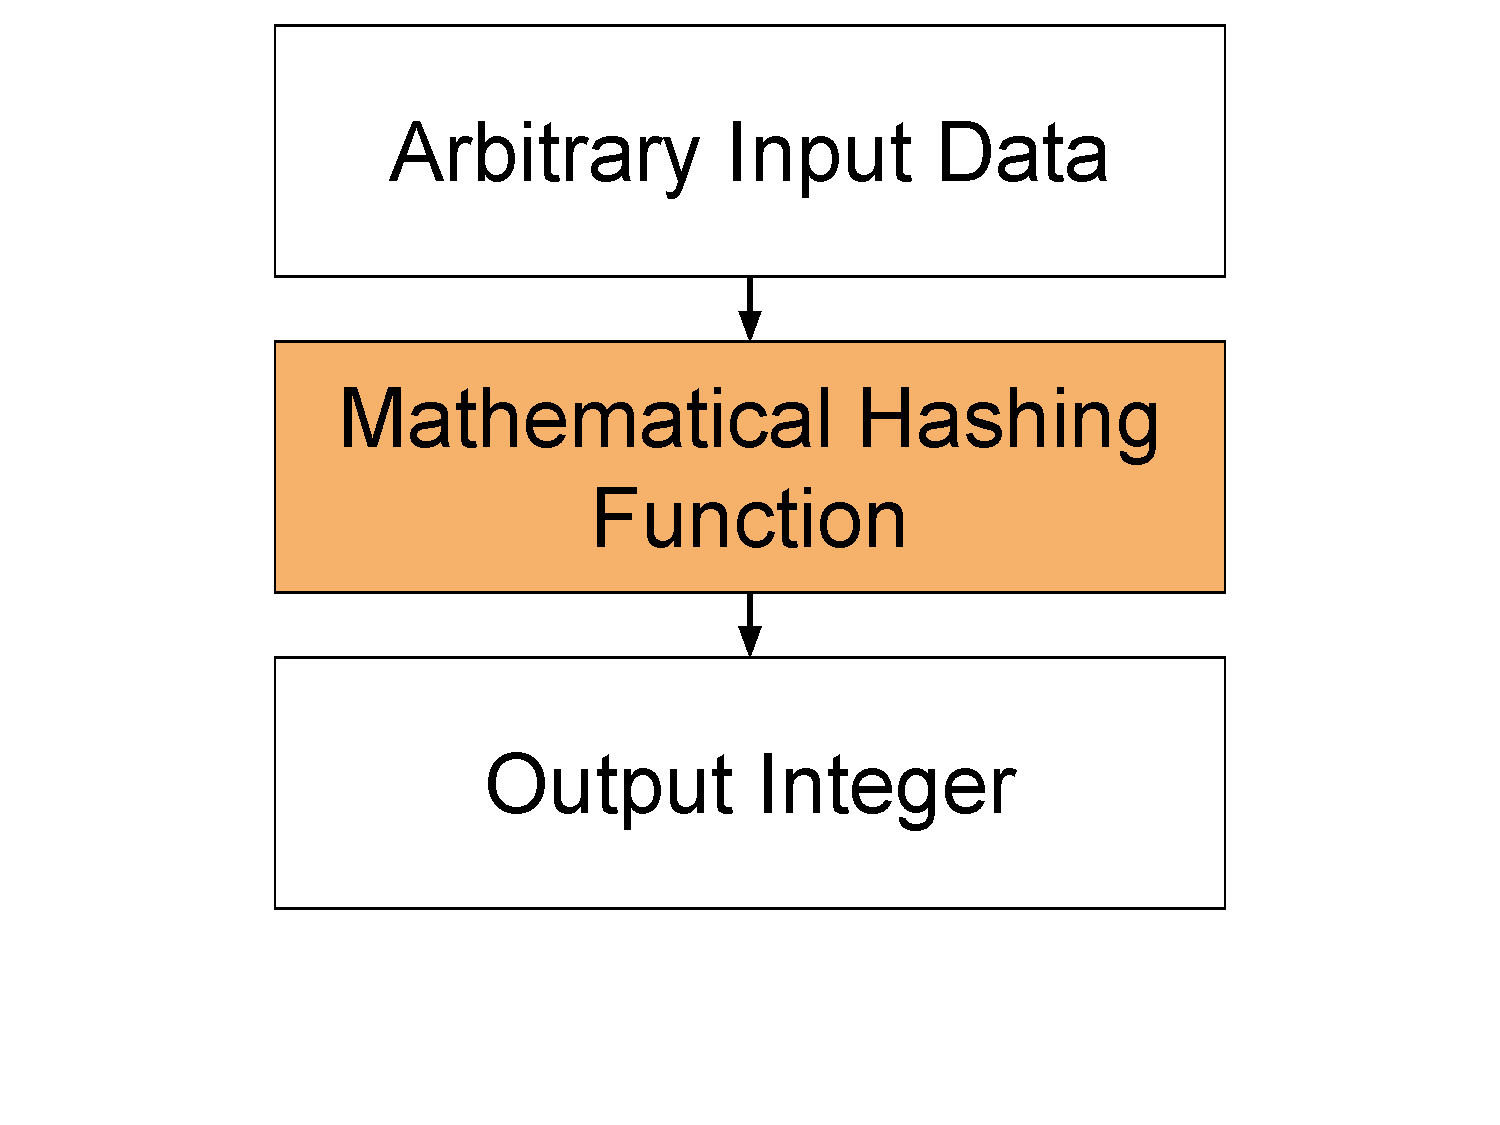
\includegraphics[width=0.8\textwidth]{./imgs/hashing.pdf}
    \vfill
\end{frame}

\begin{frame}[fragile]
    \frametitle{Hashing Values in Java}
    \begin{lstlisting}[frame=trBL]
String str1 = "Hello";
System.out.println(str1.hashCode());
    \end{lstlisting}
    \vspace{-0.25cm}
    \begin{shell}
69609650
    \end{shell}
    \hline
    \vfill
    \begin{lstlisting}[frame=trBL]
Double num = 14.5;
System.out.println(num.hashCode());
    \end{lstlisting}
    \vspace{-0.25cm}
    \begin{shell}
1076690944
    \end{shell}
    \hline
    \small
    \vspace{0.1cm}
    \textbf{Key point:} The HashValue of the values \lstinline|"Hello"| and \lstinline|14.5| are \textit{always} the same (determinitic).
\end{frame}

\begin{frame}[fragile]
    \frametitle{Hashing Custom Objects in Java}
    \begin{lstlisting}[frame=trBL]
class RandomDataContainer<E>{
    E data;
    RandomDataContainer(E data){
        this.data = data;
    }
}
RandDataContainer<String> rdc = new RandDataContainer("Hello");
System.out.println(rdc.hashCode());
    \end{lstlisting}
    \vspace{-0.2cm}
    \begin{shell}
???
    \end{shell}
    \begin{itemize}
        \item \textbf{The Issue:} The output of this will change in between each run.
        \item How do we make it deterministic?
    \end{itemize}
\end{frame}

\begin{frame}[fragile]
    \frametitle{Hashing Custom Objects in Java}
    \begin{lstlisting}[frame=trBL, basicstyle=\scriptsize]
class RandomDataContainer<E>{
    E data;
    RandomDataContainer(E data){
        this.data = data;
    }

    @Override
    public int hashCode(){
        return data.hashCode();
    }
}
RandDataContainer<String> rdc = new RandDataContainer("Hello");
System.out.println(rdc.hashCode());
    \end{lstlisting}
    \begin{minipage}{0.49\textwidth}
    \begin{shell}
69609650
    \end{shell}
    \end{minipage}
    \begin{minipage}{0.49\textwidth}
    \begin{itemize}
        \item \textbf{Key Point:} If we want an object's hashcode to be deterministic, manually override it and provide your own!
    \end{itemize}
    \end{minipage}
\end{frame}

\begin{frame}[fragile]
    \frametitle{Object Hash Purpose}
    \centering
    \textbf{Key Point:} The hashCode is used convert arbitrary objects into an integer.
\end{frame}

\begin{frame}[fragile]
    \frametitle{Index Lookup vs Hash Lookup}
    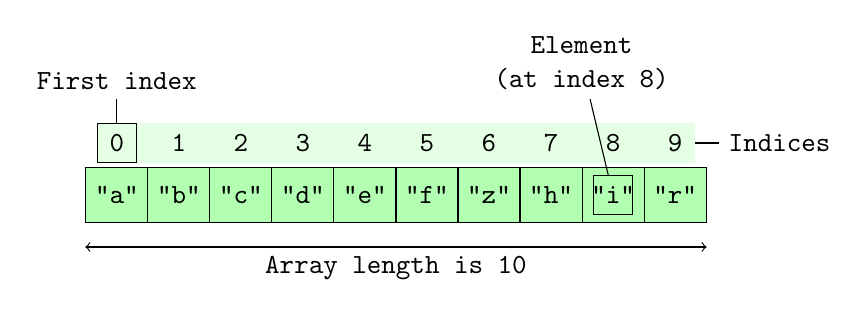
\begin{tikzpicture}[font=\ttfamily,
    array/.style={matrix of nodes,nodes={draw, minimum size=7mm, fill=green!30},column sep=-\pgflinewidth, row sep=0.5mm, nodes in empty cells,
    row 1/.style={nodes={draw=none, fill=none, minimum size=5mm}},
    row 1 column 1/.style={nodes={draw}}}]

    \matrix[array] (array) {
    0 & 1 & 2 & 3 & 4 & 5 & 6 & 7 & 8 & 9\\
    "a"  & "b"  & "c"  & "d"  & "e"  & "f"  & "z"  & "h"  & "i"  & "r" \\};
    \node[draw, minimum size=5mm] at (array-2-9) (box) {};

    \begin{scope}[on background layer]
    \fill[green!10] (array-1-1.north west) rectangle (array-1-10.south east);
    \end{scope}

    \draw[<->]([yshift=-3mm]array-2-1.south west) -- node[below] {Array length is 10} ([yshift=-3mm]array-2-10.south east);

    \draw (array-1-1.north)--++(90:3mm) node [above] (first) {First index};
    \draw (array-1-10.east)--++(0:3mm) node [right]{Indices};
    \node [align=center, anchor=south] at (array-2-9.north west|-first.south) (8) {Element\\ (at index 8)};
    \draw (8)--(box);
    %
    \end{tikzpicture}

\begin{itemize}
    \item Lookup time-complex \textit{O(1)} if we know the index of the thing that we are looking for.
    \item If we have to search it's $O(N)$ if we use an array or $O(log_2(N)$ if we switch to a tree.
    \item We can to better!
\end{itemize}
\end{frame}

\begin{frame}[fragile]
    \frametitle{Hashing to "Index"}
    \begin{enumerate}
        \item Use hashing + more math to convert a "key" to an integer.
        \item Use that integer to access an array!
        \item Creates the notion of key-value pairs.
        \item Key is the ``index'', value is the thing at that index.
    \end{enumerate}
\end{frame}

\begin{frame}[fragile]
    \frametitle{Index Lookup vs Hash Lookup}
    \resizebox{!}{0.39\textwidth}{
    \begin{figure}
        \centering
       \begin{tikzpicture}[%scale=.2,
    node distance = 7mm and 4mm,
      start chain = going right, 
       arr/.style = {semithick, -Stealth},
       dot/.style = {circle, fill, inner sep=1.2pt,
                     label=left:#1},
    every label/.append style = {font=\footnotesize, fill=white, align=center,
                                 fill opacity=0.5, text opacity=1, 
                                 inner sep=1pt},
         E/.style = {ellipse, draw, fill=#1},
      mpnh/.style = {rectangle split, rectangle split horizontal, 
                     rectangle split parts=3, draw, fill=gray!20,
                     inner sep=2pt,
                     on chain},
      mpnv/.style = {rectangle split, rectangle split parts=10,
         rectangle split part fill={gray!30,gray!10,gray!30,gray!30,gray!30,
                                    gray!10,gray!30,gray!10,gray!10,gray!30},
         draw, minimum height=2ex},
       sym/.style = {yshift=-1mm},
       syp/.style = {yshift=+1mm},
                            ]
    \node[mpnv, label=H] (H) 
        {\nodepart{one}     $\diagup$
         \nodepart{two}     \vphantom{$\diagup$} 
         \nodepart{three}   $\diagup$
         \nodepart{four}    $\diagup$
         \nodepart{five}    $\diagup$
         \nodepart{six}     \vphantom{$\diagup$} 
         \nodepart{seven}   $\diagup$
         \nodepart{eight}   \vphantom{$\diagup$} 
         \nodepart{nine}    \vphantom{$\diagup$} 
         \nodepart{ten}     $\diagup$
        };
    %
    \node[mpnh, right=of H.two east] (A1) 
       {\nodepart{one}  $\diagup$
        \nodepart{two}  $v_1$
        \nodepart{three}    \hphantom{$\diagup$}  
       };
    \node[mpnh] (A2)
       {\nodepart{one}      \hphantom{$\diagup$}
        \nodepart{two}      $v_4$
        \nodepart{three}    $\diagup$
       };
    %
    \node[mpnh, right=of H.six east] (B1)
       {\nodepart{one}      $\diagup$
        \nodepart{two}      $v_5$
        \nodepart{three}    \hphantom{$\diagup$}
       };
    \node[mpnh] (B2)
       {\nodepart{one}      \hphantom{$\diagup$}
        \nodepart{two}      $v_2$
        \nodepart{three}    \hphantom{$\diagup$}
       };
    \node[mpnh] (B3)
       {\nodepart{one}      \hphantom{$\diagup$}
        \nodepart{two}      $v_7$
        \nodepart{three}    $\diagup$ 
       };
    %
    \node[mpnh, right=of H.eight east] (C1)
       {\nodepart{one}      $\diagup$
        \nodepart{two}      $v_3$
        \nodepart{three}    $\diagup$
       };
    %
    \node[mpnh, right=of H.nine east] (D1)
       {\nodepart{one}  $\diagup$
        \nodepart{two}  $v_8$
        \nodepart{three}    \hphantom{$\diagup$}
       };
    \node[mpnh] (D2)
       {\nodepart{one}      \hphantom{$\diagup$}
        \nodepart{two}      $v_6$
        \nodepart{three}    $\diagup$
       };
    %% arrows (right)
    \draw[arr]  (H |- H.two east)   edge (A1)
                (H |- H.six east)   edge (B1)
                (H |- H.eight east) edge (C1)
                (H |- H.nine east)   to (D1)
                ;
    \draw[arr, transform canvas={yshift=1mm}]  
                (A1.three north |- A1.east)  edge (A2)
                (B1.three north |- B1.east)  edge (B2)
                (B2.three north |- B2.east)  edge (B3)
                (D1.three north |- D2)   to   (D2)
                ;
    \draw[arr, transform canvas={yshift=-1mm}]
                (A2.one north |- A2)  edge  (A1)
                (B2.one north |- B2)  edge  (B1)
                (B3.one north |- B3)  edge  (B2)
                (D2.one north |- D2)   to   (D1)
                ;
    %% dots, ellipses
    \pgfmathsetseed{3}
    Explicitly sets the seed for
    \foreach \i in {1,2,...,8}
        \node (k\i) [dot=$k_{\i}$] at (-33mm +40*rand,0.5*rand) {};


    \scoped[on background layer]
    {
    \draw[fill=gray!30]  (-4,0.4) ellipse (3 and 2);
    \path   (-4,1) node[label={$U$\\ (universe of keys)}] {};

    \draw[fill=white]   (-4,0) ellipse (2.4 and 1);
    \path   (-6,0) node[label=right:$K$\\ (actual\\ keys)] {};

    \draw[arr]  (k1)    edge ([syp] H.two west)
                (k4)    edge ([sym] H.two west)

                (k2)    edge ([syp] H.six west)
                (k5)    edge (H.six west)
                (k7)    edge ([sym] H.six west)
                
                (k3)    edge (H.eight west)
                
                (k8)    edge ([syp] H.nine west)
                (k6)    edge ([sym] H.nine west)
                ;
    }
    \end{tikzpicture}
    \end{figure}}
    \small
    \begin{itemize}
        \item The hashing algorithm produces a finite set of keys: U
        \item Our hashtable will contain a subset of those: K
        \item $k_n$ is a key that we use to index into a list.
        \item H is a list of lists where each item in the list is the hash code
    \end{itemize}
\end{frame}

\begin{frame}[fragile]
    \frametitle{Possible Uses}
    \begin{itemize}
        \item Store phone numbers:
            \begin{itemize}
                \item key: Name
                \item value: Number
            \end{itemize}
        \item Address book:
            \begin{itemize}
                \item key: Name
                \item value: Address
            \end{itemize}
        \item Dictionary:
            \begin{itemize}
                \item key: Word
                \item value: Dictionary
            \end{itemize}
    \end{itemize}
    \vfill
    \textbf{Key Takeaway:} We have key values pairs and we use to key to modify/access the value, just like an index in an array.
\end{frame}


\section{Map Interface and HashMap}

\begin{frame}[fragile]
    \frametitle{Map Interface Method}
    \begin{lstlisting}[frame=trBL]
Map<K, V> map = // ..

Map<String, Integer> map = // ..
Map<Integer, List<String>> map = // ..
    \end{lstlisting}
    \vfill
    \pause
    \begin{enumerate}
        \item \lstinline|put(K key, V value)|: Puts a key-value pair into the map.
        \item \lstinline|putAll(Map<K, V> map): Puts all of the key-value pairs into a map.
        \pause
        \item \lstinline|get(K key)|: Gets the value associated with a key in a map.
        \item \lstinline|getOrDefault(K key, V defaultValue)|: Gets the value associated with a key. If that key doesn't exist, \textit{returns the defaultValue}.
        \pause
        \item \lstinline|containsKey(K key)|: Returns true if the map contains the key and false otherwise.
        \pause
        \item \lstinline|remove(K key)|: Removes the key value pair referenced by \texttt{key}.
    \end{enumerate}
\end{frame}


\section{Iterating}
\begin{frame}[fragile]
    \frametitle{Iterating over Keys and Values}
    \begin{lstlisting}[frame=trBL]
//iterates over a maps keys
for(K key: map.keySet()){
    System.out.println(item);
}

//Iterativng over a map's values
for(V value: map.values()){
    System.out.println(item);
}
    \end{lstlisting}
    \vfill
    \begin{itemize}
        \item \lstinline|map.values()|: Gets you the collection of values present in the map.
        \item \lstinline|map.keys()|: Gets you the collection of keys in the dictionary.
    \end{itemize}
\end{frame}

\begin{frame}[fragile]
    \frametitle{Iterating over Keys-Values}
    \begin{lstlisting}[frame=trBL]
for(Map.Entry<K, V> item: map.entrySet()){
    System.out.println("Key:" +  item.getKey());
    System.out.println("Value:" +  item.getValue());
}
    \end{lstlisting}
    \vfill
    \begin{itemize}
        \item \lstinline|entrySet()|: Gives us a set of \lstinline|Map.Entry<K, V>| pairs (i.e., \lstinline|Set<Map.Entry<K, V>|).
        \item \lstinline|getKey()|: Gets you the key from a \lstinline|Map.Entry|.
        \item \lstinline|getValue()|: Gets you the value from a \lstinline|Map.Entry|.
    \end{itemize}
\end{frame}


%\section{Set}
%
%\begin{frame}[fragile]
%    \frametitle{The Set Interface}
%    \begin{lstlisting}[frame=trBL]
%Set<E> set = new HashSet<>();
%set.add("Hi");
%boolean doesContain = set.contains("Hi");
%set.remove("Hi");
%    \end{lstlisting}
%    \begin{enumerate}
%        \item \lstinline|add(E e)|: Adds an element to the set if that element isn't already in the set and returns true. If the element is already in the set this operation has no impact on the state of the set and returns false.
%        \item \lstinline|remove(E e)|: Removes an element from the set. Returns true if the element was present and removed; otherwise, returns false.
%        \item \lstinline|contains(E e)|: Returns true if the element is present in the set and false otherwise.
%    \end{enumerate}
%\end{frame}

\end{document}
